\chapter{Descrição do Problema}
\label{cap-descricao}

Decidimos escrever esse capítulo utilizando uma técnica muito útil que permite elevar a compreensão mútua de um assunto de interesse: a técnica da metáfora. 

Originalmente, as metáforas são usadas durante o desenvolvimento ágil de sistemas, na medida em que os desenvolvedores criam elementos dentro do computador para simular outros que existem regularmente fora dele, no mundo físico.  A lixeira, a mesa de trabalho, janelas, pastas e outros itens que estamos habituados a encontrar no computador, simulam elementos do mundo físico e seus respectivos comportamentos \cite{intro:metafora}.

Assim, podemos comparar a implementação de um solução de análise de dados numa instituição com uma pessoa que deseja abrir um restaurante.

\section{A Metáfora do Restaurante}
\label{sec-metafora}

Certamente, um restaurante envolve a interação harmônica entre diversos elementos. Vamos apresentar cada um deles:

\begin{itemize}
    \item \textbf{Cliente}:  A razão de existir de um restaurante é o \CLIENTE. Sem clientes um restaurante não cumpre seu propósito.

    \item \textbf{Prato}: O \PRATO \xspace é aquilo que o cliente quer consumir. Um prato é composto de ingredientes. Um exemplo de prato é o sanduíche.
    
    \item \textbf{Cardápio \& Livro de Receitas}: O \CARDAPIO \xspace é um catálogo contendo um conjunto de pratos que o cliente quer consumir.  O \LIVRODERECEITAS, por sua vez, identifica para cada prato do cardápio os ingredientes, as origens desses ingredientes (\PRODUTORES)
    e, também, explica como os ingredientes são combinados para montar o prato.
    
    \item \textbf{Ingredientes}: Um \INGREDIENTE \xspace é a unidade básica de um prato. Exemplos de ingredientes são: pão, alface, tomate, queijo, ovo. Os ingredientes juntos compõe um prato. Os seguintes elementos estão relacionados aos ingredientes:
    
    \begin{itemize}
        \item \textbf{Despensa}: \DESPENSA \xspace é o lugar dentro do restaurante onde os diversos ingredientes são armazenados de forma que estejam disponíveis quando o cozinheiro receber um pedido de preparação de prato. 
        
        \item \textbf{Produtor de ingrediente}: O \PRODUTOR \xspace é a entidade que produz um tipo específico de ingrediente. O pão vem da padaria, o alface e o tomate vem do hortifrúti e assim por diante.
    \end{itemize}

    \item \textbf{Cozinheiro}: \COZINHEIRO \xspace é a entidade responsável por preparar o prato. No exemplo do prato de sanduíche, o cozinheiro seleciona duas fatias de pão, lava o alface, corta o tomate, frita o ovo e monta o sanduíche.
    
    \item \textbf{Fogão}: \FOGAO \xspace representa todas as ferramentas que o cozinheiro utiliza para preparar os ingredientes e montar um prato. Por exemplo: Ele usa uma faca para fatiar o tomate, usa o fogo para fritar o ovo, que certamente não é servido cru, etc... 
    
    \item \textbf{Gerente}:  \GERENTE \xspace é a pessoa responsável por assegurar que cada elemento do restaurante cumpra com sua função. Por exemplo, se o prato servido não agrada o cliente, então o cliente reclama com o gerente que deve, por sua vez, verificar porque isso ocorre. Pode ser que o cozinheiro não saiba preparar o prato ou pode ser que ele não disponha das ferramentas necessárias para fazer isso. Cabe ao gerente avaliar as situações e agir.
\end{itemize}

Certamente, o leitor já deve estar imaginando que elementos do mundo real da análise de dados são correspondentes aos elementos fictícios da metáfora apresentada. Vamos discutir cada um.

\subsection*{Cliente}
\label{sub-cliente}
    Na metáfora apresentada o \CLIENTEDORESTAURANTE \xspace representa o \textbf{usuário final} que consumirá as informações e utilizará essas informações para tomar decisões e agir.
    
    Em última instância, os clientes são as entidades que exercem a competência de fiscalizar. Conforme afirma \cite[20]{propostaCDDHCEDP}, a competência de fiscalização na CLDF é em grande parte exercida pelas Comissões Permanentes e Comissões Temporárias. Ainda, o cidadão também pode fiscalizar e, portanto, o cidadão também é um cliente.
    
    São muitos clientes potenciais. E precisamos começar em algum lugar. Então, por diversas razões, que estão descritos na \emph{proposta}\footnote{A partir deste momento, para simplificar, vamos passar a nos referir à ``Proposta para Modernização da Função Institucional de Fiscalização no âmbito da Comissão de Defesa dos Direitos Humanos, Cidadania, Ética e Decoro Parlamentar, com Aplicação Computacional de Ciência de Dados \& BI'' \cite{propostaCDDHCEDP} com o termo em itálico: ``\emph{proposta}''.}[página 22], o cliente foi definido como sendo a \textbf{Comissão de Defesa dos Direitos Humanos, Cidadania, Ética e Decoro Parlamentar (CDDHCEDP)}.
    
    \begin{env-destaque}{Cliente identificado!}
        O \CLIENTE \xspace é a \textbf{Comissão de Defesa dos Direitos Humanos, Cidadania, Ética e Decoro Parlamentar (CDDHCEDP)}.
    \end{env-destaque}

\subsection*{Prato}
\label{sub-prato}

    O \PRATO \xspace representa a \textbf{necessidade de informação do cliente}. Não estamos falando do dado bruto, mas sim do produto de inteligência gerado através da combinação de diversos dados. A figura \ref{fig:intro:dadostoinfo} mostra o processo de transformação de dados brutos em inteligência passando pela informação. 
    
    \begin{figure}[h]
        \centering
        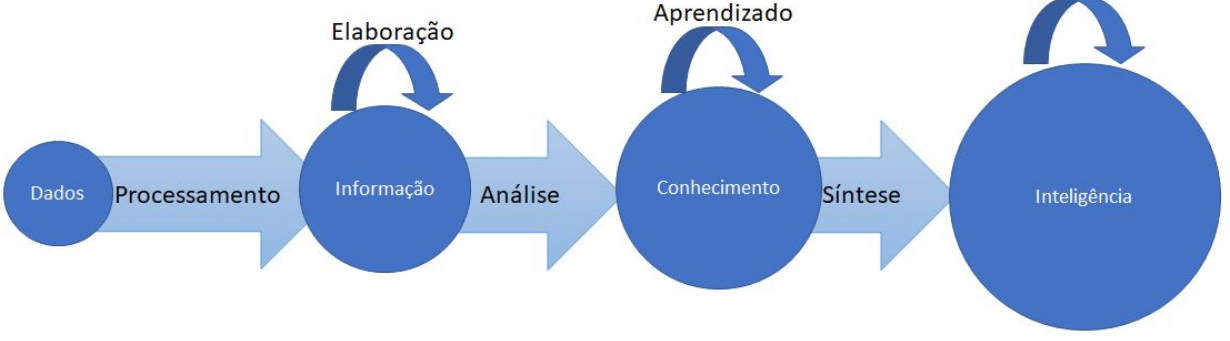
\includegraphics[width=0.9\textwidth]{fig/fig-dadostoinfo.png}
        \caption{Criação de inteligência a partir de dados. Fonte: \cite{propostaCDDHCEDP}}
        \label{fig:intro:dadostoinfo}
    \end{figure}    
    
    Vamos usar a \emph{proposta} para dar um exemplo de prato, isto é, de informação que o \CLIENTE \xspace gostaria de consumir:
    
    \begin{env-exemplo}{Exemplo de \PRATO}
        Necessidade de informação: Quantidade de pessoas que foram atendidas em algum Centro de Referência da Assistência Social do Distrito Federal (CRAS) no último ano que também estão inscritas no ``Programa Bolsa Família'' do Governo Federal.
    \end{env-exemplo}
    
\subsection*{Cardápio de Pratos}
\label{sub-cardapio}

    O \CARDAPIO \xspace é um catálogo contendo um conjunto de pratos, que vão satisfazer um determinado cliente. Trata-se de um \textbf{levantamento de necessidades de informação} necessárias para satisfazer as demandas.
    
    A ``Proposta para Modernização da Função Institucional de Fiscalização no âmbito da Comissão de Defesa dos Direitos Humanos, Cidadania, Ética e Decoro Parlamentar, com Aplicação Computacional de Ciência de Dados \& BI'' \cite{propostaCDDHCEDP} apresenta um riquíssimo cardápio de pratos\footnote{Na \emph{proposta}, os \PRATOS \xspace correspondem aos indicadores de direitos humanos. Ao todo foram levantados 5 (cinco) conjuntos de indicadores, perfazendo um total de 169 (cento e sessenta e nove) indicadores específicos e mais 45 (quarenta e cinco) indicadores gerais para serem utilizados em cruzamentos de dados.}. 
    
    \begin{env-destaque}{Cardápio de Pratos elaborado!}
        O \CARDAPIO \xspace é a \textbf{``Proposta para Modernização da Função Institucional de Fiscalização no âmbito da Comissão de Defesa dos Direitos Humanos, Cidadania, Ética e Decoro Parlamentar, com Aplicação Computacional de Ciência de Dados \& BI''}.
    \end{env-destaque}    
    
\subsection*{Ingredientes}
\label{sub-ingredientes}

    O \INGREDIENTE, por sua vez, representa o \textbf{dado bruto}. A informação é criada através do processamento de diferentes dados. 
    
    Vamos usar o Exemplo de \PRATO \xspace apresentado para identificar \textbf{de forma hipotética} os dados que seriam necessários para gerar a informação requisitada.

    \begin{env-exemplo}{Exemplos de \INGREDIENTES}
    
        \textbf{Dados requeridos para necessidade de informação}: Quantidade de pessoas que foram atendidas em algum Centro de Referência da Assistência Social do Distrito Federal (CRAS) no último ano que também estão inscritas no ``Programa Bolsa Família'' do Governo Federal.
    
        \begin{itemize}
            \item \textbf{Ingrediente 1:} 
            Tabela contendo registros das pessoas que foram atendidas na CRAS BRASÍLIA;
            
            \item \textbf{Ingrediente 2:} 
            Tabela contendo registros das pessoas que foram atendidas na CRAS BRAZLÂNDIA;
            
            \item (...)
            
            \item \textbf{Ingrediente 27\footnote{De acordo com \cite{intro:cras}, o Distrito Federal possui 27 CRAS organizados por territórios.}:} Tabela contendo registros das pessoas que foram atendidas na CRAS VARJÃO;

            \item \nohyphens{\textbf{Ingrediente 28:} Tabela contendo o cadastro das pessoas inscritas no ``Programa Bolsa Família'';}
        \end{itemize}
    \end{env-exemplo}    
    
    Dessa forma, precisamos de 28 ingredientes para produzir a informação desejada. Veja que ainda não especificamos como esses ingredientes devem ser combinados para montar o prato, ou seja, não especificamos a origem desses dados e nem definimos como os dados devem ser processados para gerar a informação.
    
    \subsection*{Despensa}
    \label{sub-despensa}

    Embora o exemplo anterior apresentou apenas os \INGREDIENTES \xspace necessários para produzir o prato desejado, o conjunto de ingredientes necessários para produzir todos os pratos de um cardápio é muito maior. Assim, os diversos ingredientes necessários para produzir os mais variados pratos precisam ser armazenados em algum lugar. A \DESPENSA \xspace é o local onde os ingredientes são armazenados.
    
    No mundo real, a despensa representa os \textbf{armazéns de dados}, isto é, o \textbf{repositório de dados analíticos.}
    
    De certo, quando você vai preparar um sanduíche, você não utiliza todos os ingredientes da sua despensa. Por outro lado, não importa o quanto abarrotado de alimentos a sua despensa está, não se monta um sanduíche sem seus ingredientes específicos. O mesmo acontece na análise de dados. Algumas informações dependem de um conjunto de dados específico cuja ausência impede que aquela informação seja produzida.
    
    \subsection*{Produtor de Ingrediente}    
    O \PRODUTOR \xspace representa a \textbf{fonte de dados}. Deseja-se  identificar as organizações que armazenam dados de interesse. 
    
    Algumas instituições reúnem e oferecem os dados ao público por meio de APIs\footnote{A sigla API refere-se ao termo em inglês ``\emph{Application Programming Interface}'' que significa em tradução para o português ``Interface de Programação de Aplicativos''. Trata-se de um conjunto de rotinas e padrões de programação para acesso a um aplicativo de software ou plataforma baseado na Web \cite{wikipedia:api}.}. Outros dados de interesse podem estar contidos em sistemas informatizados. Ainda, inúmeros dados encontram-se em formatos de dados não estruturados\footnote{Dados não estruturados são compostos por qualquer combinação de conteúdos textuais, de imagens, voz ou da web \cite[70]{turban2019}.}.
    \index{API}
    \index{Dados não estruturados}
    
    \subsection*{Livro de Receitas}
    \label{sub-livrodereceitas}
    
    Enquanto o cardápio de pratos apenas elenca um conjunto de pratos que o cliente gostaria de consumir. O \LIVRODERECEITAS \xspace identifica, para cada prato, quais ingredientes são necessários, quais os produtores desses ingredientes e quais as metodologias e processos devem ser usados para preparar os ingredientes e montar o prato.
    
    No mundo real, o livro de receitas representa o \textbf{processamento dos dados}. A seguir apresentamos um exemplo de receita.
    
    \begin{env-exemplo}{Exemplo de \RECEITA}
        \begin{enumerate}
            \item \emph{\textbf{Especificação dos Ingredientes (Dados):}}
                \begin{itemize}
                    \item \textbf{Ingrediente 1:} Tabela contendo registros de pessoas que foram atendidas na CRAS BRASÍLIA;
                    \item \textbf{Ingrediente 2:} Tabela contendo registros de pessoas que foram atendidas na CRAS BRAZLÂNDIA;
                    \item (...)                
                    \item \textbf{Ingrediente 27:} Tabela contendo registros de pessoas que foram atendidas na CRAS VARJÃO;
                    \item \textbf{Ingrediente 28:} Tabela contendo o cadastro das pessoas inscritas no ``Programa Bolsa Família'';  
                \end{itemize}
            \item \emph{\textbf{Produtores dos Ingredientes (Fontes de Dados):}}
                \begin{itemize}
                    \item Origem dos Ingredientes 1 a 27: Secretaria de Desenvolvimento Social do GDF;
                    \item Origem do Ingrediente 28: Secretaria Especial do Desenvolvimento Social do Ministério da Cidadania;
                \end{itemize}
            \item \emph{\textbf{Preparação dos Ingredientes (Processamento dos Dados):}}
                \begin{enumerate}
                    \item Criar tabela contendo a união de todos os registros de todas as tabelas de CRAS;
                    \item Filtrar apenas os registros de atendimentos realizados no último ano;
                    \item Selecionar todas as pessoas que aparecem na tabela de pessoas inscritas no ``Programa Bolsa Família'' que também aparecem na tabela união filtrada;
                    \item Contar total de registros;
                \end{enumerate}
        \end{enumerate}
    \end{env-exemplo}    

\subsection*{Cozinheiro}
\label{sub-cozinheiro}

    O \COZINHEIRO \xspace representa os \textbf{cientistas e analistas de dados} responsáveis por utilizar as ferramentas para fazer o processamento e transformar os dados em informações.
    
    Aqui é importante comentar a respeito dos ``tipos'' de cozinheiros, ou seja, dos modelos possíveis para que o trabalho operacional seja realizado:
    
    \begin{itemize}
        \item \textbf{``Cozinheiros da Casa''}: Servidores da CLDF com capacidade técnica para fazer esse trabalho. Esses profissionais podem ser tanto servidores da CMI quanto servidores representantes das unidades organizacionais clientes (Comissões Permanentes e outras unidades interessadas) treinados e capacitados para operar as ferramentas. 

        \item \textbf{``Cozinheiros Contratados''}: Representa uma empresa contratada para prestar esse tipo de serviço especializado de extração dos dados, transformação, limpeza, manipulação, cruzamento, criação e configuração dos artefatos (\emph{dashboards}, alertas, etc...) contendo os ``pratos'', isto é, as informações requisitadas pelos clientes.
    \end{itemize}

    Cada modelo apresenta condições, vantagens e desvantagens.
    
    A condição de termos ``Cozinheiros da Casa'' realizando o trabalho operacional necessário é o investimento em cursos de treinamento e capacitação. A vantagem é que os
    ativos de conhecimento são mantidos na casa. Outra vantagem ocorre quando os ``cozinheiros'' são representantes dos próprios clientes, treinados e capacitados para utilizar as ferramentas e produzir as informações. 
    
    A desvantagem é que o quadro de servidores efetivos é muito reduzido e já é bastante atarefado com as atividades de suas unidades. Além disso, nem todos os potenciais clientes possuem representantes dispostos a realizar o treinamento necessário. Finalmente, algumas tarefas como os processos de extração, transformação e carregamento dos dados são tarefas complexas até para os usuários mais experientes. 
    
    Assim, o modelo que se sugere é o modelo híbrido formado pela combinação de ``Cozinheiros da Casa'' e ``Cozinheiros Contratados''. 

\subsection*{Fogão}
\label{sub-fogao}

    O \FOGAO \xspace representa o \textbf{conjunto de produtos de software e hardware}, que serão utilizados pelos cientistas e analistas de dados no processo de acesso, transformação, tratamento, preparação, limpeza dos dados e as atividades de processamento necessárias para transformá-los em informação, que será apresentada, reportada, consultada, afinal, consumida pelos clientes. De certo, uma das contribuições deste estudo é na identificação e avaliação desses produtos de acordo com as necessidades específicas dessa casa legislativa.

\subsection*{Gerente}
\label{sub-gerente}

    Os \GERENTES \xspace representam os \textbf{Servidores da CLDF} responsáveis por garantir que todos os elementos cooperem entre si. O gerente deve ser treinado pois precisa conhecer todos os aspectos de funcionamento do restaurante. Precisa entender o que satisfaz os clientes, precisa saber trabalhar com o fogão, deve ser capaz de fiscalizar a atuação dos cozinheiros, etc. 


    Para referência, a tabela \ref{tab:intro:metafora} mostra a correspondência entre elementos da metáfora e do mundo real.

    \begin{table}[htbp]
        \begin{center}
        \begin{tabular}{|c|c|c|}
            \hline
                % NOME DA TABELA        
                \rowcolor{cldfB1} \multicolumn{2}{|c|}{\Large \METAFORADORESTAURANTE} \\  
                \rowcolor{cldfB1} \multicolumn{2}{|c|}{\large \textbf{Tabela Resumo}} \\ \hline \hline
                % CABEÇALHO        
                \rowcolor{lightgray}\textbf{Elementos da Metáfora} & \textbf{Elementos do Mundo Real} \\ \hline
                % CONTEÚDO
                % Código gerado pela tabela do Google SpreadSheets Cenário GA
                \rowcolor{cldfC!30}\CLIENTE & Usuário Final \\ \hline
                \rowcolor{cldfD!30}\PRATO & Necessidade de Informação \\ \hline
                \rowcolor{cldfC!30}\CARDAPIO & Levantamento de Necessidades de Informação \\ \hline
                \rowcolor{cldfD!30}\INGREDIENTE & Dado Bruto \\ \hline
                \rowcolor{cldfC!30}\DESPENSA & Repositório de Dados Analíticos \\ \hline
                \rowcolor{cldfD!30}\PRODUTOR & Fonte de Dados \\ \hline
                \rowcolor{cldfC!30}\LIVRODERECEITAS & Rotinas de Processamento dos Dados \\ \hline
                \rowcolor{cldfD!30}\COZINHEIRO & Cientistas e Analistas de Dados \\ \hline
                \rowcolor{cldfC!30}\FOGAO & Ferramentas de software e hardware \\ \hline
                \rowcolor{cldfD!30}\GERENTES & Servidores da CLDF \\ \hline
        \end{tabular}    
        \caption{\label{tab:intro:metafora} Correspondência entre elementos da metáfora e o mundo real}
        \end{center}
    \end{table}

% ----------------------------------------------------------------------------------

\section{Cenários Possíveis}

Nessa seção pretendemos usar a \METAFORADORESTAURANTE \xspace descrita anteriormente para apresentar situações e cenários possíveis. 

% Só apresentar e quando não satisfeito deixar perguntas em aberto.

\subsection{Cenário: Não temos um Cliente bem definido}    


    % Usar a seguinte estrutura. Descreve-se o cenário antes do box e descreve-se a realidade depois.

    A primeira situação hipotética é o de não haver nenhum \CLIENTE \xspace para nosso \RESTAURANTE. Isto é, o primeiro cenário é o de não ser necessário abrir o restaurante pois ninguém está interessado em consumir produtos dele.
    
    \begin{env-cenario}{Cenário: Não existe Cliente}
            \mschecknao \xspace \CLIENTE 
    \end{env-cenario}
    
    Sabemos que este não é o caso pois conforme apresentado na seção \ref{sub-cliente} temos um cliente bem definido: a CDDHCEDP. Além disso, há ainda mais 10 Comissões na CLDF que constituem um amplo conjunto de futuros clientes potenciais.
    
\subsection{Cenário: Não sabemos o que o Cliente quer}    
    
    Neste cenário, temos \CLIENTES \xspace potenciais mas não sabemos que \PRATOS \xspace eles querem consumir.
    
    \begin{env-cenario}{Cenário: Não sabemos o que o Cliente quer}
            \mschecksim \xspace \CLIENTE  
            
            \mschecknao \xspace \CARDAPIO
    \end{env-cenario}

    Novamente, de acordo com a seção \ref{sub-cardapio} sabemos que este cenário já foi superado pois a \emph{proposta} representa um rico cardápio de pratos.

\subsection{Cenário: Não sabemos preparar os Pratos}    
    
    Temos \CLIENTES \xspace potenciais, criamos um \CARDAPIO \xspace e, portanto, sabemos o que querem consumir, mas não identificamos os \INGREDIENTES, tampouco os \PRODUTORES. Ou seja, não temos um \LIVRODERECEITAS  \xspace com as \RECEITAS  \xspace para preparar os \PRATOS.
    
    \begin{env-cenario}{Cenário: Não sabemos preparar os Pratos}
            \mschecksim \xspace \CLIENTE 
            
            \mschecksim \xspace \CARDAPIO

            \mschecknao \xspace \LIVRODERECEITAS
    \end{env-cenario}
    
    Em síntese, um \LIVRODERECEITAS \xspace não será necessário caso os clientes sejam eles mesmos capazes de utilizar as ferramentas e produzir as informações. No entanto, quando esse não é o caso, o que fazer nessa situação?

\subsection{Cenário: Não temos Fogão}

    Temos \CLIENTES \xspace potenciais, sabemos o que eles querem consumir, sabemos preparar os pratos, mas não temos as ferramentas para fazer isso.

    \begin{env-cenario}{Cenário: Não temos Fogão}
            \mschecksim \xspace \CLIENTE 
            
            \mschecksim \xspace \CARDAPIO  

            \mschecksim \xspace \LIVRODERECEITAS
            
            \mschecknao \xspace \FOGAO
    \end{env-cenario}

    Um dos objetivos deste estudo é justamente entender e analisar comparativamente ferramentas de análise de dados de diferentes fornecedores.


\subsection{Cenário: Não temos Cozinheiros capacitados ou contratados}    

    Neste cenário temos um \CLIENTE \xspace identificado, sabemos o que ele quer, dispomos de um \LIVRODERECEITAS, temos \FOGAO, mas não temos \COZINHEIROS \xspace capazes de preparar os pratos.

    \begin{env-cenario2}{Cenário: Não temos Cozinheiros capacitados ou contratados}
            \mschecksim \xspace \CLIENTE 
            
            \mschecksim \xspace \CARDAPIO  

            \mschecksim \xspace \LIVRODERECEITAS
            
            \mschecksim \xspace \FOGAO

            \mschecknao \xspace \COZINHEIROS \xspace capacitados ou contratados
    \end{env-cenario2}
    
    Certamente, o \PRATO \xspace não se monta sozinho. Os dados devem ser combinados e passar por um processamento para que a informação seja gerada.

\subsection{Cenário: Não temos Gerentes treinados}   

     Temos um \CLIENTE \xspace identificado, sabemos o que ele quer, sabemos preparar o prato, temos \FOGAO \xspace e até temos uma equipe de \COZINHEIROS \xspace capacitados ou contratados, mas não temos \GERENTES \xspace capazes de cuidar do restaurante.

    \begin{env-cenario2}{Cenário: Não temos Gerentes Treinados}
            \mschecksim \xspace \CLIENTE 
            
            \mschecksim \xspace \CARDAPIO  

            \mschecksim \xspace \LIVRODERECEITAS
            
            \mschecksim \xspace \FOGAO

            \mschecksim \xspace \COZINHEIROS \xspace capacitados ou contratados
        
            \mschecknao \xspace \GERENTES \xspace treinados
    \end{env-cenario2}

    Como saber se o cozinheiro está realizando o seu trabalho corretamente se o próprio gerente não entende do serviço?

\subsection{Cenário: Não temos Despensa}
\label{sub-cenario-naotemosdespensa}

    Outro cenário é o de não termos despensa, isto é, um local seguro para armazenar os ingredientes.

    \begin{env-cenario2}{Cenário: Não temos Despensa}
            \mschecksim \xspace \CLIENTE 
            
            \mschecksim \xspace \CARDAPIO  

            \mschecksim \xspace \LIVRODERECEITAS
            
            \mschecksim \xspace \FOGAO

            \mschecksim \xspace \COZINHEIROS \xspace capacitados ou contratados
        
            \mschecksim \xspace \GERENTES \xspace treinados

            \mschecknao \xspace \DESPENSA
    \end{env-cenario2}

    Certamente, com a ampliação do número de clientes atendidos pelo restaurante, maior quantidade de diferentes ingredientes serão necessários para preparar os diferentes pratos. Esses ingredientes devem ser armazenados em um lugar seguro de forma que sua qualidade e integridade sejam preservadas e ainda estejam disponíveis toda vez que cozinheiros autorizados quiserem utilizá-los para preparar novos pratos. 

\subsection{Cenário: Não temos Ingredientes}
\label{sub-cenario-naotemosingredientes}

    \begin{env-cenario2}{Cenário: Não temos Ingredientes}
            \mschecksim \xspace \CLIENTE 
            
            \mschecksim \xspace \CARDAPIO  

            \mschecksim \xspace \LIVRODERECEITAS
            
            \mschecksim \xspace \FOGAO

            \mschecksim \xspace \COZINHEIROS \xspace capacitados ou contratados
        
            \mschecksim \xspace \GERENTES \xspace treinados

            \mschecksim \xspace \DESPENSA

            \mschecknao \xspace \INGREDIENTES
    \end{env-cenario2}

    Certamente este é o pior cenário que poderia acontecer porque ele significa que recursos foram investidos na aquisição de ferramentas de software e hardware, cientistas e analistas de dados foram contratados, os servidores foram treinados, mas o cliente ainda não tem suas necessidades de informação satisfeitas porque os dados para produzir as informações não estão disponíveis, não foram identificados, não são acessíveis ou não existem. 
    
    Outro comentário é a importância de os ingredientes satisfazerem os pratos solicitados pelo cliente. Ou seja, de nada adianta o cliente solicitar um sanduíche e você entregar um pão com manteiga porque a despensa não dispõe de todos os ingredientes necessários para montar o prato que ele pediu. 

\section{Cenário Ideal}
\label{sec-cenarioideal}

    \begin{env-cenario2}{Cenário Ideal}
            \mschecksim \xspace \CLIENTE 
            
            \mschecksim \xspace \CARDAPIO  

            \mschecksim \xspace \LIVRODERECEITAS
            
            \mschecksim \xspace \FOGAO

            \mschecksim \xspace \COZINHEIROS \xspace capacitados ou contratados
        
            \mschecksim \xspace \GERENTES \xspace treinados

            \mschecksim \xspace \DESPENSA

            \mschecksim \xspace \INGREDIENTES
    \end{env-cenario2}

    Finalmente, este é o cenário ideal buscado, que exibe todas as condições para uma implementação de sucesso de um ambiente de análise de dados numa organização.
    
    Neste cenário, o Cliente foi identificado. Sabemos o que ele quer. Sabemos preparar os pratos. Dispomos de ferramentas. Temos cozinheiros capacitados dentro da organização para realizar o trabalho ou terceirizamos esse serviço contratando cozinheiros. Os gerentes entendem como o restaurante funciona e como os diferentes elementos se integram. E, mais importante, dispomos dos ingredientes específicos, armazenados numa despensa, para que seja possível montar os pratos do cardápio e satisfazer o cliente.

    % INTRODUZ PRÓXIMO CAPITULO
    O próximo capítulo vai apresentar a estrutura deste estudo desenvolvido para buscar atingir esse cenário.